\begin{frame}{Overview}{Architecture}
    Our system includes: \pause a \textbf{Portal}, \pause a distributed file storage system \textbf{IPFS} \pause and a private blockchain network \textbf{Hyperledger Fabric}.
    \pause
    \begin{figure}
        \centering
        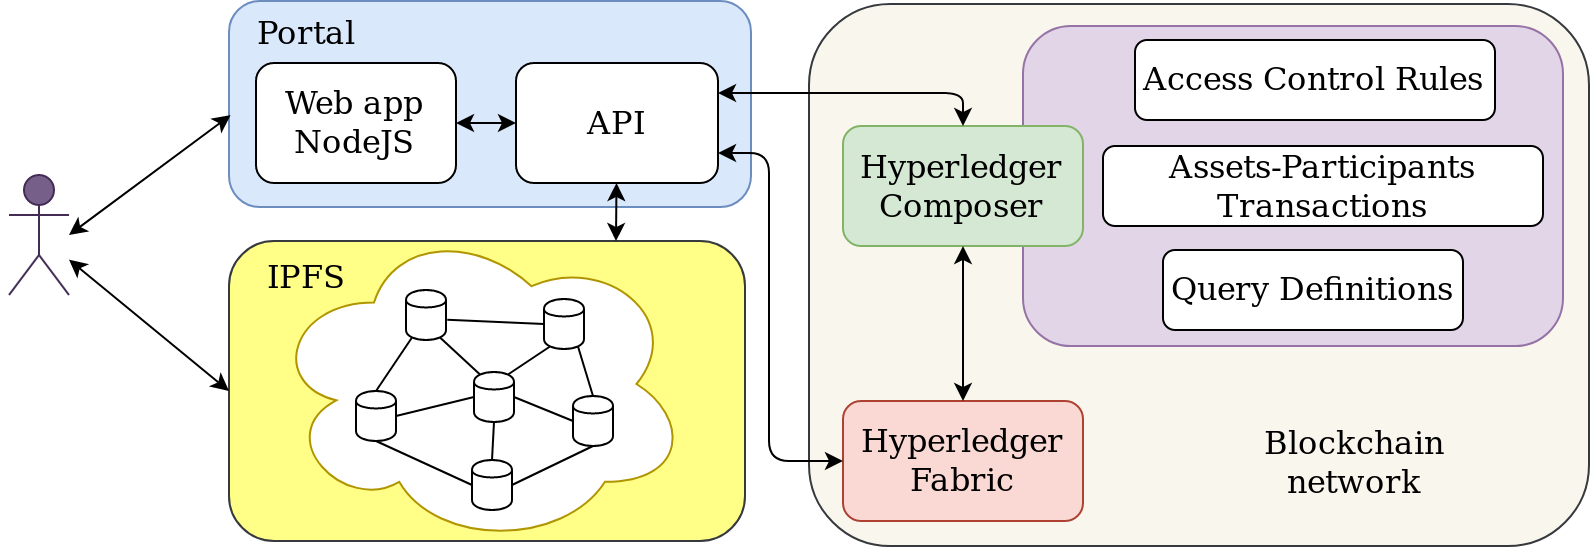
\includegraphics[width=.9\textwidth,height=0.4\textwidth]{img/ArOv.png}
        % \caption{Architecture overview}
        % \label{fig:arOv}
    \end{figure}
\end{frame}

\begin{frame}{Overview}{Explaining}
    Why Hyperledger Fabric and IPFS?
    \setbeamercovered{transparent}
    \begin{itemize}
        \uncover<2->{\item We want to decentralize our system as much as we can.}
              \uncover<3->{\item Hyperledger Fabric: authenticates data contributor, traces data log, checks data integrity, enhances the system transparency.}
              \uncover<4->{\item IPFS: ensures the data integrity and availability.}
    \end{itemize}
\end{frame}



% \begin{frame}{Overview}{Modules role}
%     \setbeamercovered{transparent}
%     \begin{itemize}
%         \onslide<1->{
%         \item[1.] The \textbf{Portal} \textit{handles user requests}:
%               % is responsible for interacting with two remaining parts.
%               \begin{itemize}
%                   %   \uncover<2->{
%                   %   \item<2-> handles user requests;
%                   %   }
%                   % \uncover<3->{
%                   \item<2-> Triggering smart contracts.
%                         % }
%                         % \uncover<4->{
%                   \item<3-> Uploading data to the IPFS.
%                         % }
%               \end{itemize}
%               }
%               \pause
%               \pause
%               \pause
%               %   \pause
%               \onslide<4->{
%         \item[2.] The \textbf{IPFS} \textit{enhances the data integrity and availability}:
%               \begin{itemize}
%                   \uncover<5->{
%                   \item Storing the data sets.
%                         }
%                         \uncover<6->{\item Generating the content-based address.}
%                         % \uncover<8->{\item enhances the data integrity and availability.}
%               \end{itemize}
%               }
%               %     \end{itemize}
%               % \end{frame}

%               % \begin{frame}{ Overview}
%               %     \setbeamercovered{transparent}
%               %     \begin{itemize}
%               \pause
%               \pause
%               \pause
%               %   \pause
%               \onslide<7->{
%         \item[3.] The \textbf{Hyperledger Fabric} \textit{improves system transparency, enhances integrity and manages system}:
%               % plays an important role in ensuring transparency and enhancing the data integrity.
%               \begin{itemize}
%                   \uncover<8->{\item Storing the metadata of the data sets.}
%                         \uncover<9->{\item Authenticating data contributors.}
%                         % \uncover<12->{\item enhances the system transparency;}
%                         \uncover<10->{
%                         % \item Providing a mechanism to distributed verify all data content.
%                   \item Distributed verifying data content.
%                         }
%               \end{itemize}
%               }
%     \end{itemize}
% \end{frame}

% \begin{frame}{ Hyperledger Fabric network}
%     The general structure of Hyperledger Fabric network:
%     \begin{figure}
%         \centering
%         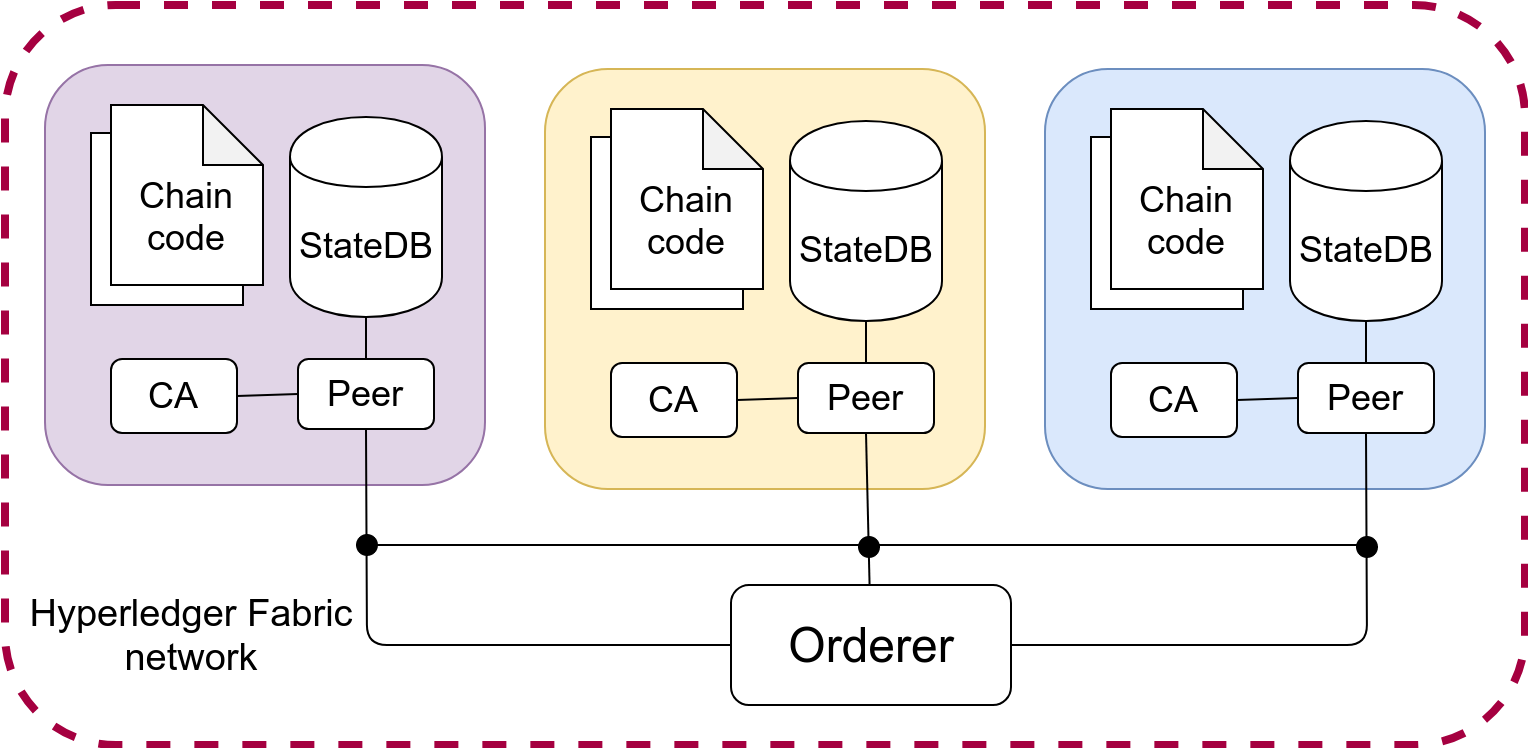
\includegraphics[width=.8\textwidth]{img/HFnet.png}
%         % \caption{Architecture overview}
%         % \label{fig:netArchi}
%     \end{figure}
% \end{frame}

% \begin{frame}{ Hyperledger Fabric network}
%     In the structure of the network, \textbf{organization}s represent ministries that contribute data to the open data portal.
%     \setbeamercovered{transparent}
%     \begin{itemize}
%         \uncover<2->{\item \textbf{Peers} participates in network operation.}
%               \uncover<3->{\item \textbf{Certificate Authority} issues and authenticates digital certificates.}
%               \uncover<4->{\item \textbf{Local database} includes \textit{world state} and \textit{blockchain ledger}.}
%               \uncover<5->{\item \textbf{Chaincode}.}
%     \end{itemize}
% \end{frame}


% \begin{frame}{ Hyperledger Fabric network}
%     \setbeamercovered{transparent}
%     \begin{itemize}
%         \onslide<1->{\item[+] \textbf{Chaincode}
%               \begin{itemize}
%                   \uncover<2->{\item handles business logic;}
%                         \uncover<3->{\item defines types of transactions, access control rules, type of participants, type of assets and custom queries;}
%                         \uncover<4->{\item triggers transactions to store metadata, user identity, and log events into the blockchain ledger and the distributed databases.}
%               \end{itemize}
%               }
%               \pause
%               \pause
%               \pause
%               \pause
%               \onslide<5->{\item[+] \textbf{Endorsement Policy} defines the number of node participating in the consensus process.}
%     \end{itemize}
% \end{frame}


\begin{frame}{System features}
    Our system has two main features:
    \begin{itemize}
        \item Publishing the data sets.
        \item Downloading-Verifying the data sets.
    \end{itemize}
\end{frame}

\begin{frame}{System features}{Publishing the data sets}
    \begin{center}
        \begin{figure}[H]
            \resizebox{0.8\linewidth}{!}{
                \begin{sequencediagram}
                    \renewcommand\unitfactor{0.5}
                    \newthread{B}{\textsf{Data Publisher}}{}
                    \newinst[1]{D}{\textsf{Server}}
                    \newinst[1]{F}{\textsf{IPFS}}
                    \newinst[1]{E}{\textsf{Hyperledger Fabric network}}
                    \begin{call}{B}{\textsf{Verify()}}{D}{result}
                    \end{call}
                    \begin{sdblock}{\textsf{alt}}{result=token}

                        \begin{call}{B}{\textsf{pubFunc()}}{D}{\textsf{return}}
                            \begin{call}{D}{\textsf{Authen()}}{E}{\textsf{result}}
                            \end{call}
                            \begin{sdblock}{alt}{result=true}
                                \begin{call}{D}{\textsf{upload()}}{F}{\textsf{data address}}
                                \end{call}
                                \begin{call}{D}{\textsf{pubTransac()}}{E}{\textsf{return}}
                                \end{call}
                            \end{sdblock}
                        \end{call}
                    \end{sdblock}
                \end{sequencediagram}}
            % \caption{The publishing data sets process.}
            % \label{fig:publishDataset}
        \end{figure}
    \end{center}
\end{frame}


\begin{frame}{System features}{Downloading-verifying the data sets}
    \begin{center}
        \begin{figure}[H]
            \resizebox{0.7\linewidth}{!}{
                \begin{sequencediagram}
                    \newthread{A}{\textsf{Citizens}}
                    \newinst[1]{D}{\textsf{Server}}
                    \newinst[1]{C}{\textsf{IPFS}}
                    \newinst[1]{E}{\textsf{Hyperledger Fabric network}}
                    \begin{call}{A}{\textsf{access()}}{D}{\textsf{return}}
                        \begin{call}{D}{\textsf{queryAllDatasets()}}{E}{\textsf{return}}
                        \end{call}
                    \end{call}
                    \begin{call}{A}{\textsf{downFunc()}}{D}{\textsf{return address}}
                        \begin{sdblock}{opt}{check data integrity}
                            \begin{call}{A}{\textsf{isDataValid()}}{D}{\textsf{return}}
                                \begin{call}{D}{\textsf{download()}}{C}{\textsf{return}}
                                \end{call}
                                \begin{call}{D}{\textsf{VerifyData()}}{E}{\textsf{return}}
                                \end{call}
                            \end{call}
                        \end{sdblock}
                    \end{call}
                    \begin{call}{A}{\textsf{download()}}{C}{\textsf{return}}
                    \end{call}
                \end{sequencediagram}}
            % \caption{The downloading-verifying process.}
            % \label{fig:downloadData}
        \end{figure}
    \end{center}
\end{frame}